\documentclass[12pt,twocolumn]{article}



%\usepackage[utf8]{inputenc}
\usepackage{amsmath}
%\usepackage{ae}
\usepackage{graphicx}
\usepackage{color}
\usepackage{bbm}
\usepackage[swedish]{babel}
\newcommand{\N}{\ensuremath{\mathbbm{N}}}
\newcommand{\Z}{\ensuremath{\mathbbm{Z}}}
\newcommand{\Q}{\ensuremath{\mathbbm{Q}}}
\newcommand{\R}{\ensuremath{\mathbbm{R}}}
\newcommand{\C}{\ensuremath{\mathbbm{C}}}
\newcommand{\rd}{\ensuremath{\mathrm{d}}}
\newcommand{\id}{\ensuremath{\,\rd}}
\newcommand{\ket}[1]{|#1\rangle}
\newcommand{\bra}[1]{\langle#1|}
\newcommand{\braket}[2]{\bra{#1}#2\rangle}
\newcommand{\bracket}[3]{\bra{#1}#2\ket{#3}}

\title{adsf}
\author{}
\newpage

\begin{document}
\tableofcontents
\renewcommand{\abstractname}{Abstract}
\begin{abstract}
\end{abstract}
\section{Introduction}

\section{Experimental setup}
In this experiment we used two plastic scintillator detectors located on top of each other with a gap of 2.4 meters. Below the lowest one we also had a barrel. See fig(). When a muon goes through one of the scintillator detectors we will get a pulse that is amplified by a photo multiplier. By then measuring the time difference between pulses from respective detector we can determine the speed of the muons. We also placed a radiactive $^{60}$Co sample below the lowest detector for calibration, since it releases two photons at the same time and we can thus capture the event when the photons gets absorbed in different detectors. The pulses from the two detectors were delayed in such a way that these two measurements could be done at the same time.\newline

To determine the lifetime of the muons we used on scintillator and the barrel detector. Coincidence between the barrel and the scintillator were used to be able to identify signals from muons that went through the scintillator and then absorbed in the barrel. The barrel will first give a signal from the energy absorbed when slowing down the muon and another signal when it decays. The start and stop signals are separated by an AND respectively AND-NOT gate with the scintillator signal, see fig().



\section{Results}
To determine the lifetime of the muon we fitted an exponential distribution to the measured data. However, the Time To Amplitude converter could not measure very well for small and large lifetimes, thus we only considered a limited interval $[t_1,t_2]$ and this has to be taken into account into the propability distribution. By looking at the spectrum it is reasonable to also add a constant noise $C$, so the distribution is
\begin{equation}
f(t)=\frac{\exp{(-t/\tau)}+C}{\tau\exp{(-t_1/\tau)}-\tau\exp{(-t_2/\tau)}+C(t_2-t_1)}\label{pdf}
\end{equation}

To determine $\tau$ and $C$ for our measured data the likelyhood function $\prod f(t_i)$ was minimized yielding $\tau=2.0$ $\mu$s and $C=0.05$. \newline

The statistical error was determined by sampling many different simulated sets of data points by using the distribution \eqref{pdf} and then calculate the standard deviation of these sets. The likelyhood function was also calculated to see that it was consistent with the likelyhood function for the real data points, thus verifying the validity of the model. \newline

By applying the same method it is also possible to verify that the obtained constant noise is not just statistical fluctuations. Minimizing the likelyhood function with respect to the lifetime and the constant noise set to zero a lifetime of $2.21$ $\mu$s is obtained. Using this lifetime to sample new sets of data points, and then fitting the distribution \eqref{pdf} to these data points it is possible to obtain the expected size of the statistical noise. This gives a simulated mean noise of $1.3\cdot 10^{-4}$ with standard deviation $9.4\cdot 10^{-5}$ compared to the noise of the data which is about $0.0021$. It is thus clear that this can not be explained by statistical fluctuations and must be taken into account in the model.


\section{Conclusions}
The obtained lifetime for the muon is slightly lower than the accepted value of $2.2$ $\mu$s which is not even in our error margin. However, this can be explained by the fact that there are two muons, $mu^+$ and $\mu^-$, which doesnt have the same lifetimes in the detector material \cite{}. $\mu^+$ has the same lifetime as in vacuum, while $\mu^-$ has a lifetime of about $2.0$ $\mu$s. The size of the measurement data obtained in this experiment is too small to be able to separate these two exponential distributions.


% Figurer inkluderade som eps-filer
%% \begin{figure}\centering
%% 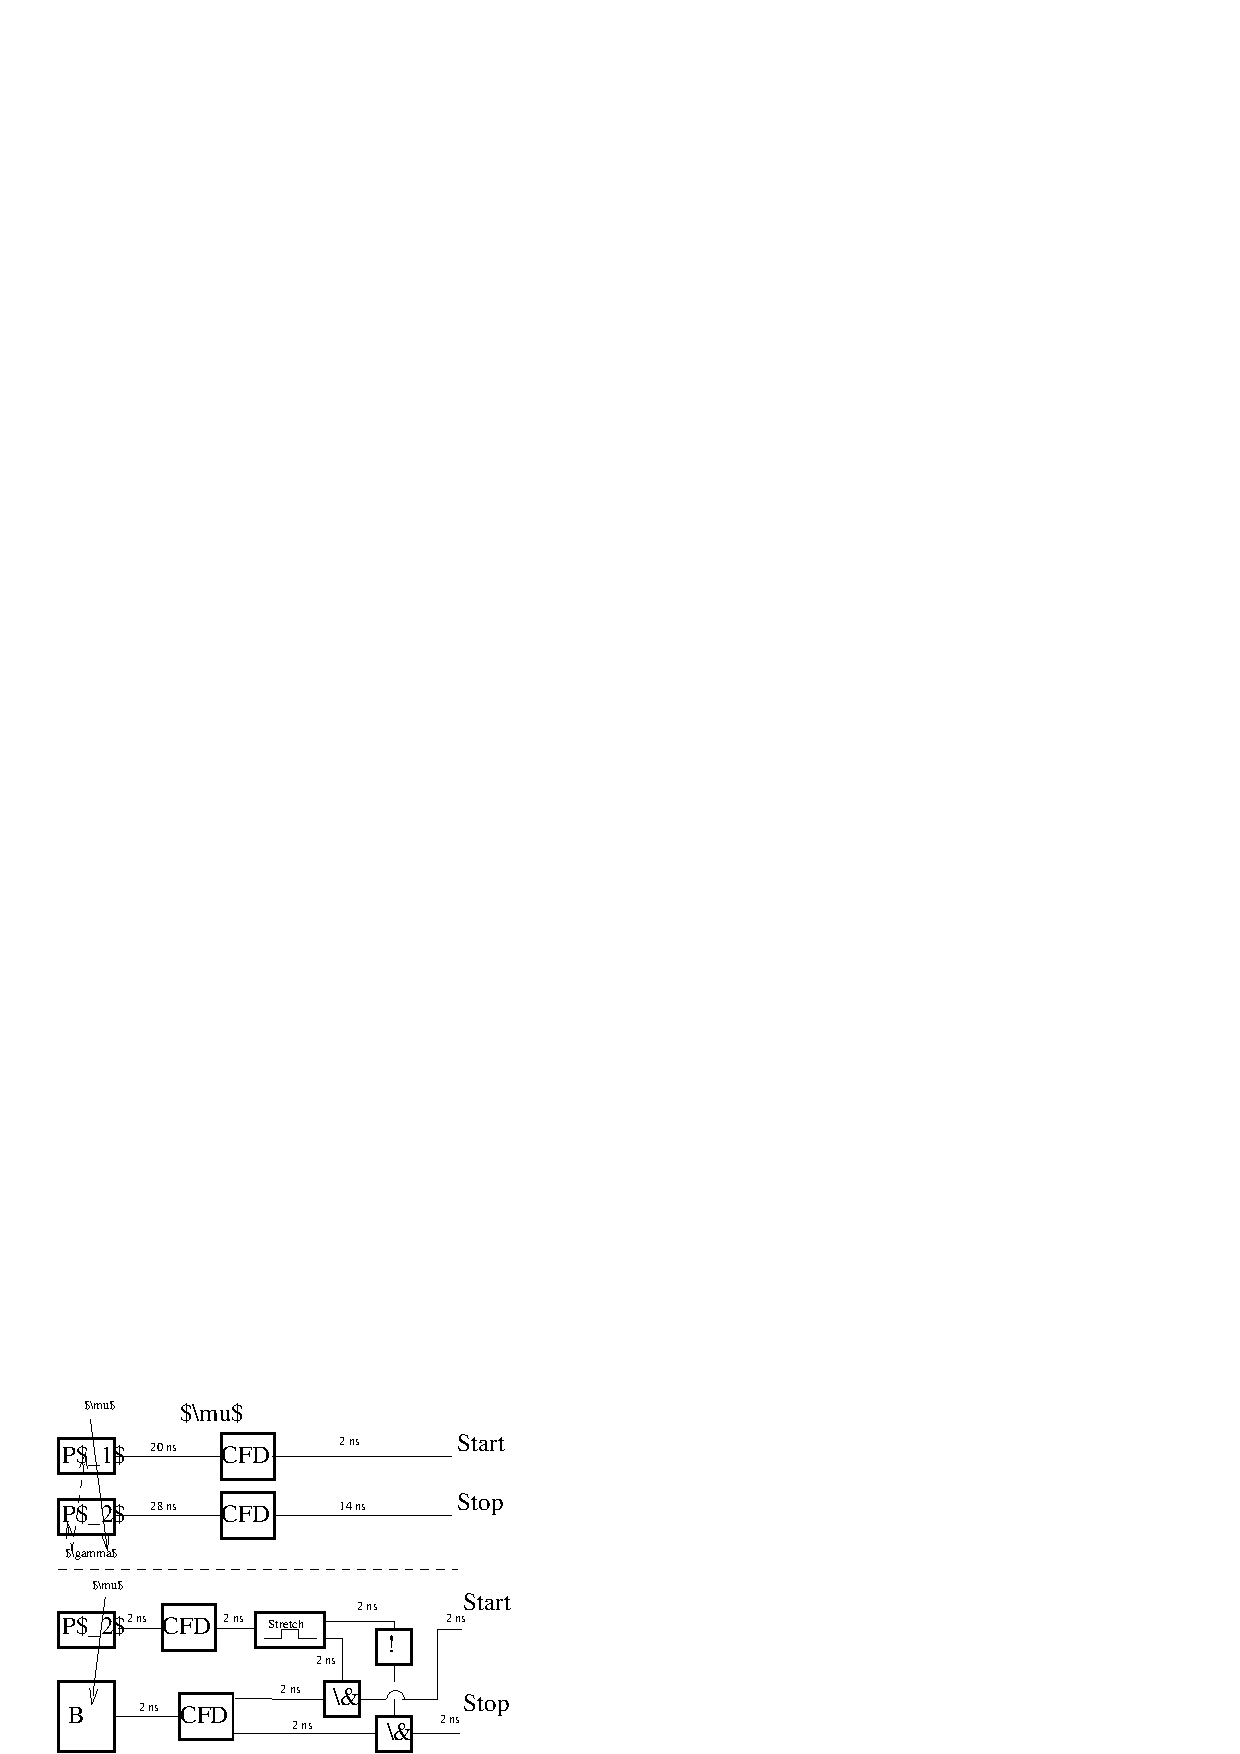
\includegraphics{speed.pdf}
%% \caption{\label{figuren} Perioden $T$ som funktion av pendellängden.}
%% \end{figure}

% Figurer inkluderade med xfigs postscript+latex

\begin{figure}[h]
\input{speed.pspdftex}
\caption{\label{setup} Schematic diagram of the different operations acting on the input signals.}
\end{figure}

\end{document}
